%!TEX root = ../../terrainbook.tex
% chktex-file 46

\graphicspath{{appendices/equations/figs/}}

\chapter{Some useful equations}%
\label{app:equations}

%%%
%
\section{Centre of a circle defined by 3 points}%
\label{sec:centrecircle}


% https://web.archive.org/web/20161011113446/http://www.abecedarical.com/zenosamples/zs_circle3pts.html
% https://web.archive.org/web/20210506191306/http://www.ambrsoft.com/trigocalc/circle3d.htm
% https://math.stackexchange.com/questions/213658/get-the-equation-of-a-circle-when-given-3-points

\begin{kaobox-info}
  This section is taken and adapted from:
  \\
  \url{https://www.ambrsoft.com/trigocalc/circle3d.htm}
\end{kaobox-info}


\begin{marginfigure}
  \centering
  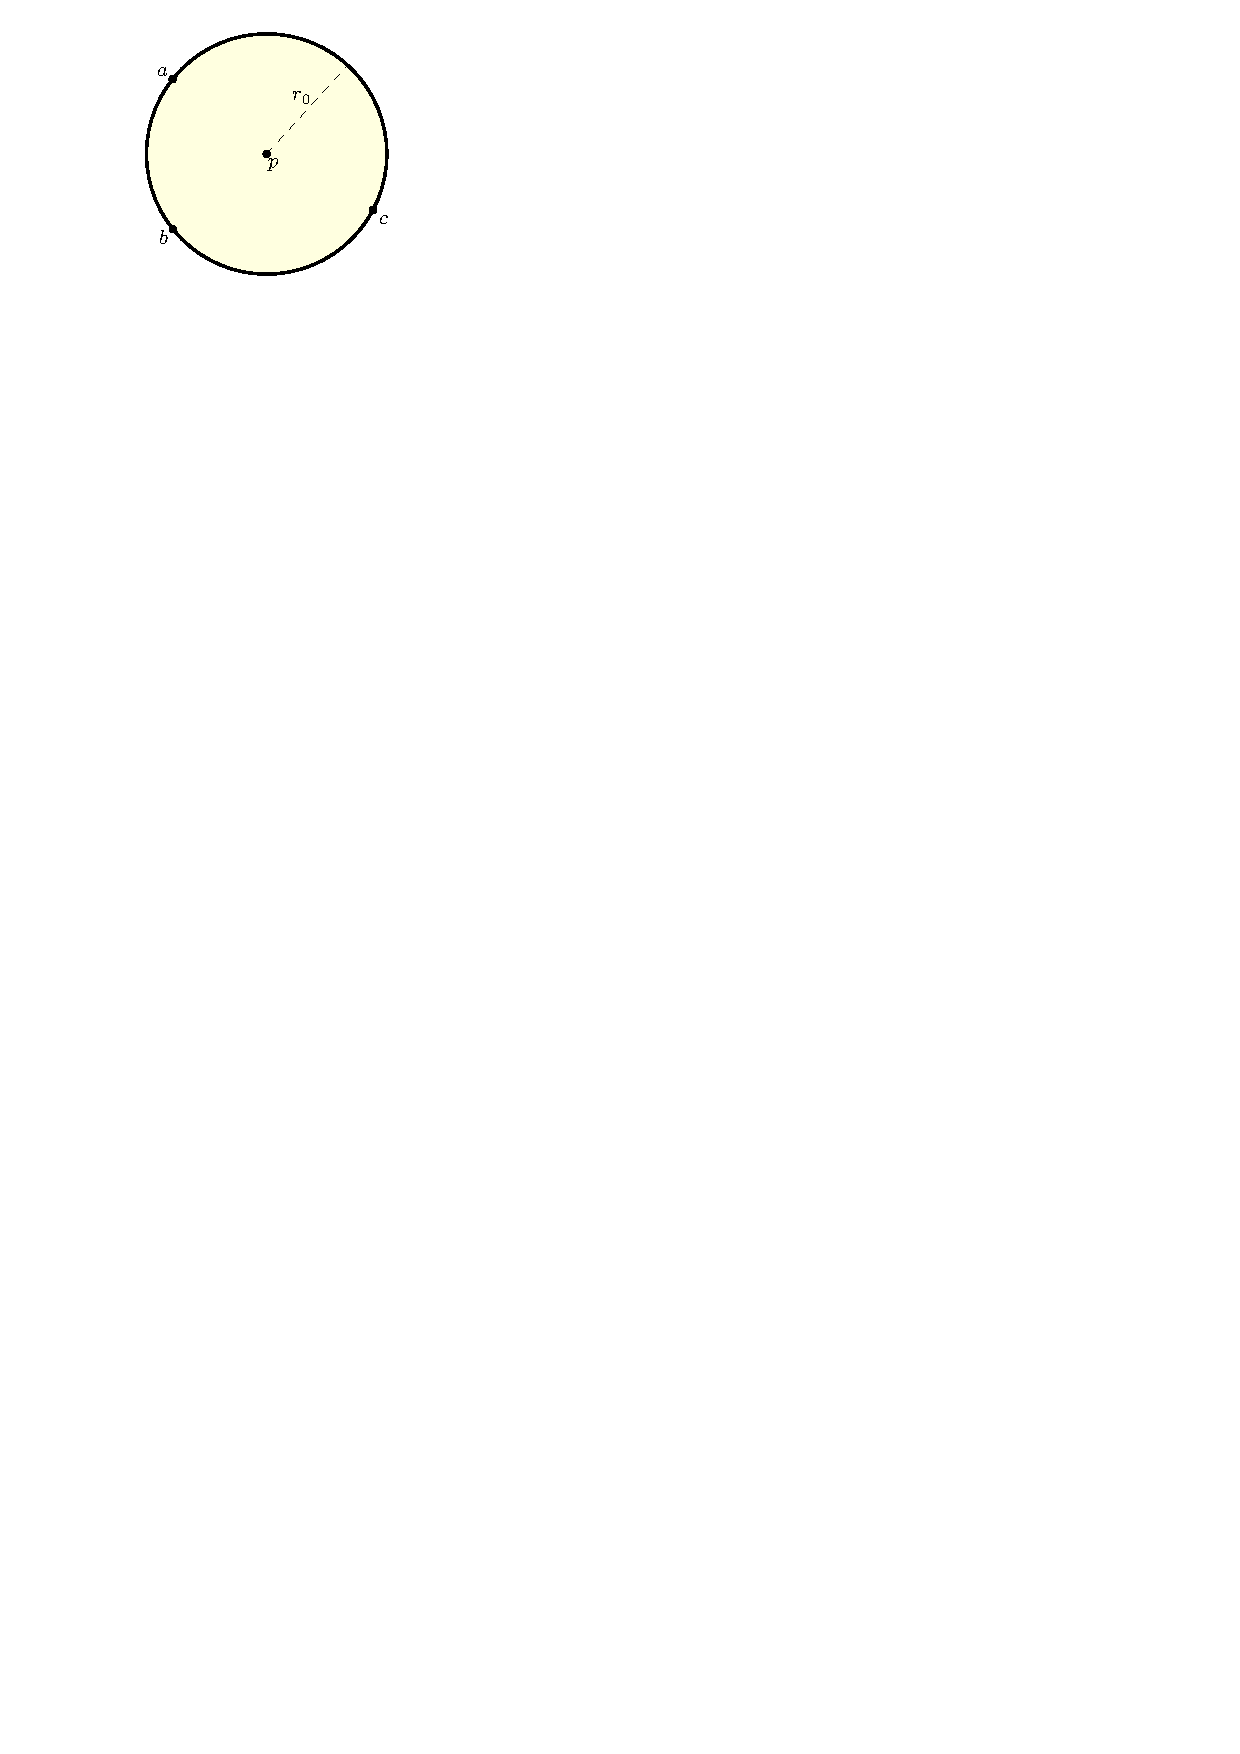
\includegraphics[width=\linewidth]{circle.pdf}
\end{marginfigure}


Given the 3 points $a$, $b$, and $c$ in the plane, we can determine the unique circle passing through those 3 points by solving the following determinant equation:
\begin{equation}
  \left| 
  \begin{array}{cccc}
    x^2 + y^2 & x & y & 1 \\
    a_x^2 + a_y^2 & a_x & a_y & 1 \\
    b_x^2 + b_y^2 & b_x & b_y & 1 \\
    c_x^2 + c_y^2 & c_x & c_y & 1 \\
  \end{array} 
  \right| 
  = 0
\end{equation}

We can rewrite the determinant as:
\begin{equation}
  (x^2 + y^2)M_{11} - xM_{12} + yM_{13} - M_{14} = 0
\end{equation}
where $M_{ij}$ is a minor of the 4x4 matrix.

The general equation of a circle is $x^2 + y^2 = r^2$, which means:
\begin{equation}
  r^2 - x\frac{M_{12}}{M_{11}} + y\frac{M_{13}}{M_{11}} - \frac{M_{14}}{M_{11}} = 0
\end{equation}

For a circle with centre $p$ and radius $r_p$, its general equation is:
\begin{equation}
  (x - p_x)^2 + (y - p_y)^2 = r_p^2
\end{equation}
if we expand and rearrange:
\begin{equation}
  r^2 - 2xp_x - 2yp_y + p_x^2 + p_y^2 -r_p^2 = 0
\end{equation}

Thus:
\begin{equation}
  p_x = \frac{M_{12}}{2M_{11}}
\end{equation}
\begin{equation}
  p_y = \frac{M_{13}}{2M_{11}}
\end{equation}
\begin{equation}
  r_p^2 = \frac{M_{14}}{M_{11}} + p_x^2 + p_y^2
\end{equation}